\begin{abstract}
TODO
\end{abstract}

\chapter{Einleitung}
Moderne Computerspiele setzen meistens auf eine graphische Darstellung ihrer Spielwelt. Dabei geht vor allem in den letzten Jahren der Trend  verstärkt in die Richtung fotorealistischen 3D-Renderings und weg von der simpleren 2D Darstellung.
Dabei ist schnelles 2D-Rendering immer noch eine nichttriviale Aufgabe für GPUs. Für viele Anwendungen sind die verfügbaren Bibliotheken im Allgemeinen immer noch viel zu langsam. Um das zu verbessern, haben wir mit \textit{BunnySuite} ein Framework entwickelt, mit dem gängige 2D-Grafik-Bibliotheken einem automatisierten Stresstest ausgesetzt werden können.\\
Mit dem \textit{BunnyMark}\footnote{https://github.com/openfl/openfl-samples/tree/master/demos/BunnyMark} gab es bereits eine Metrik zum Vergleich von Bibliotheken. Jedoch wurde hier nur die Anzahl der gerenderten Objekte (in diesem Fall Häschen, deshalb der Name) gemessen, bei denen noch 60 fps erreicht werden. Diese Zahl war nur schwer zu interpretieren und musste für ein ausführlicheres Ranking durch aussagekräftigere Metriken, bspw. \textit{Renderzeit pro Frame bei X Objekten} ersetzt werden. Auch findet diese Messung bei BunnyMark zu Demozwecken nur interaktiv statt: Häschen werden per Mausklick zur Szene hinzugefügt. Im von uns entwickelten BunnySuite-Framework können solche Messungen automatisiert erfolgen. Die Tests für mehrere Frameworks werden automatisch nacheinander gestartet und das Ergebnis wird in einem Diagramm zusammengefasst. Das Framework ist leicht erweiterbar, so dass man es mit wenig Aufwand an neue Bibliotheken anpassen kann.\\
Das vollautomatisierte Test-Framework soll Entscheidern der Spieleentwicklung die Möglichkeit eines Rankings bieten, um die richtige Bibliothek für ihre Anforderungen zu finden. Des Weiteren sollen Entwickler von Bibliotheken das Framework nutzen können, um ihre eigene Engine zu testen und zu optimieren. Die Leistungen der Bibliotheken können so transparent verglichen werden, was den Wettbewerb zwischen den Bibliotheken stimulieren und Anreize setzen soll, stärker an der Performanz zu arbeiten.

\chapter{Zeitplan und Aufgabenverteilung}
Das Team hat sich darauf geeinigt, dass jeder Entwickler sich auf eine Bibliothek konzentriert. In regelmäßigen Meetings werden Konzepte diskutiert und Designentscheidungen getroffen. Auf diese Weise soll in allem Frameworks eine vergleichbare Implementierung erreicht werden.\\
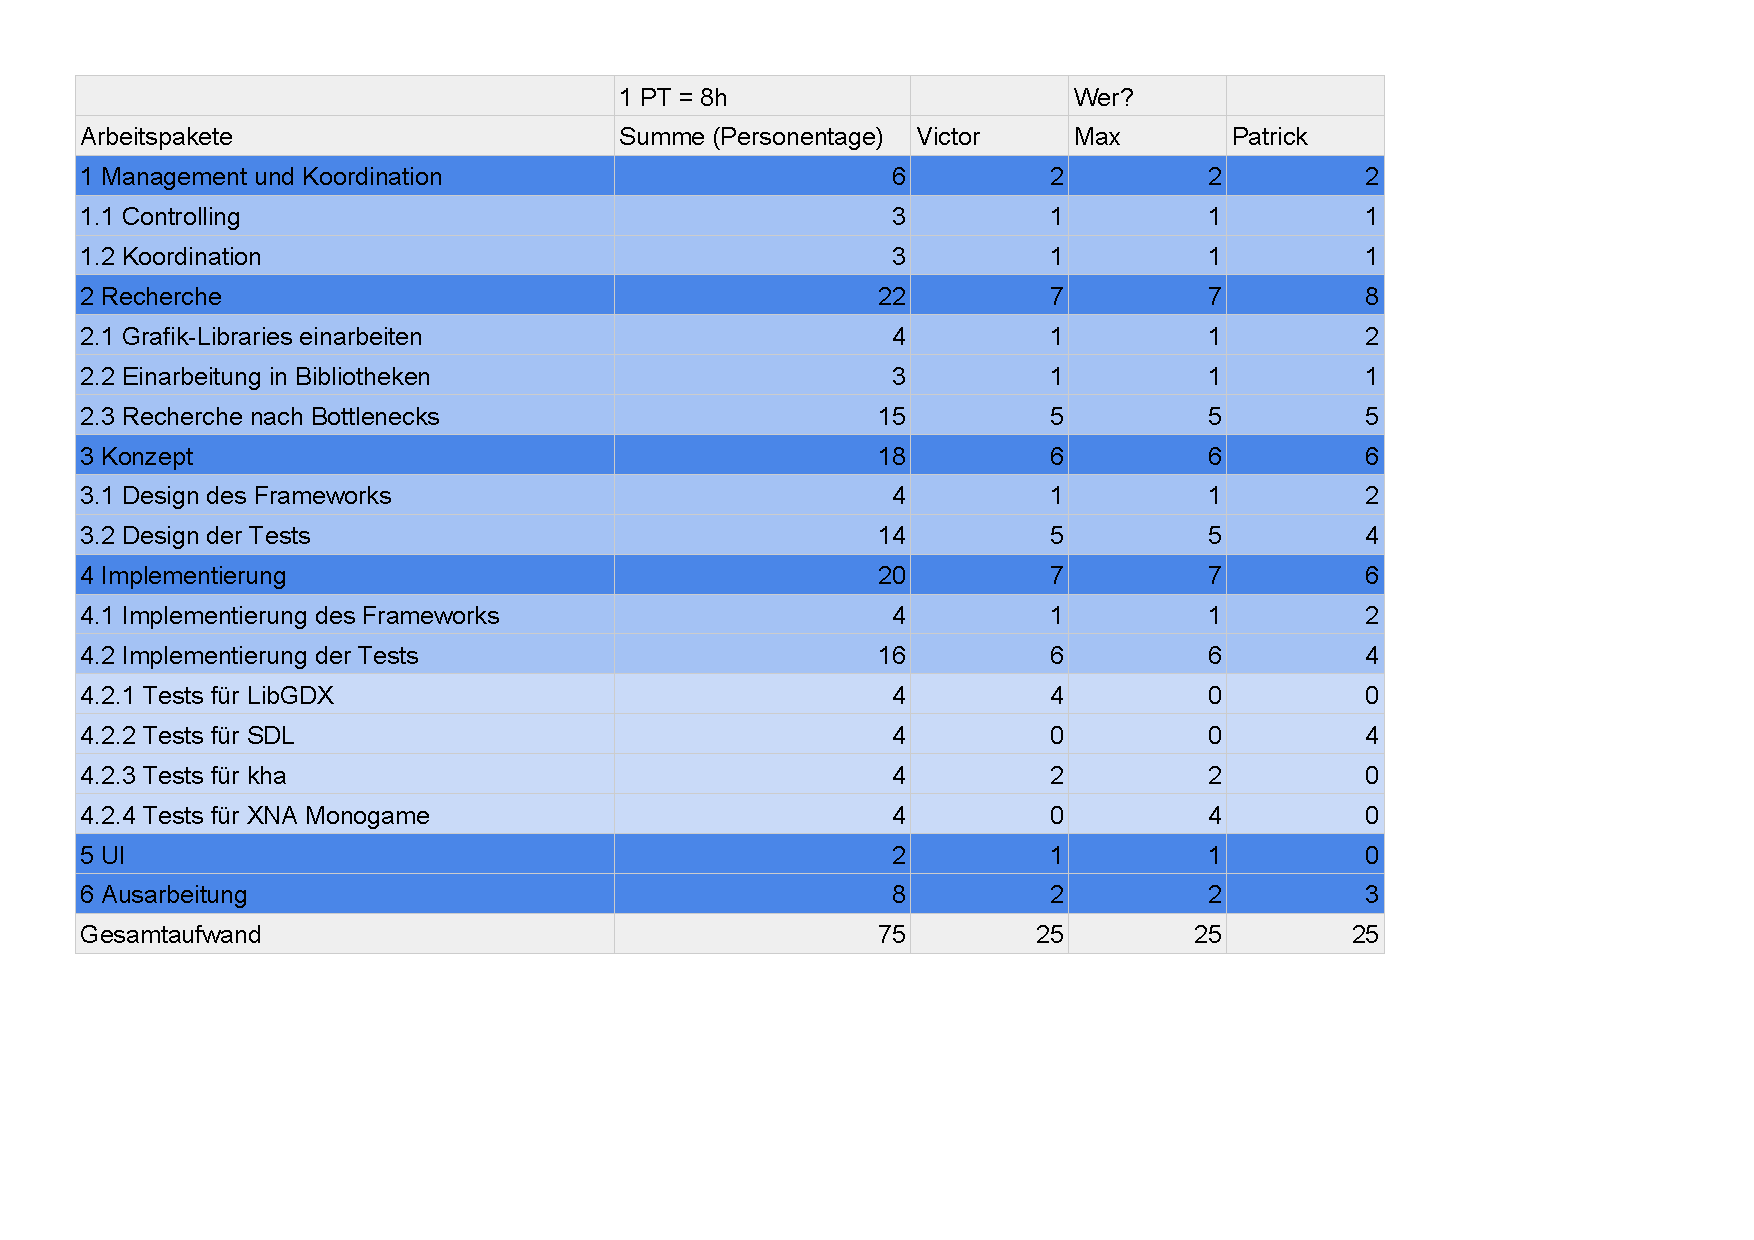
\includegraphics[width=1.2\textwidth]{projektplan.pdf}


\chapter{Grundlagen}
\section{2D-Frameworks}
Game-Frameworks sollen die Entwickler beim Implementieren der Game-Loop unterstützen. Diese Game-Loop besteht hauptsächlich aus 2 Phasen:

\begin{description}
\item[Update()] Der interne Zustand der Spielwelt und ihrer Objekte wird aktualisiert, beispielsweise die Position der Spielfigur gemäß der Benutzereingaben angepasst oder das nächste Frame in einer Animation wird ausgewählt oder die Punktzahl erhöht. Zeitgleich finden hier auch komplexere Berechnungen statt, wie die Kollisionsbestimmung, die wieder zu neuen Berechnungen führen kann (Positionen werden angepasst, damit Objekte sich nicht überlagern; "Gesundheitswerte" werden bei Treffern verringert).\\
\item[Draw()] Die im vorherigen Schritt berechnete Spielwelt wird auf dem Bildschirm dargestellt. Dazu gehören die korrekte Position aller Objekte, die Texturierung und Beleuchtung dieser Objekte, und gegebenenfalls Transformationen (Skalierung, Rotation). Auch muss bei Überlagerung von Objekten auf die korrekte Darstellung geachtet werden. Dies gilt auch für verdeckte Rückseiten von Objekten. Anschließend wird noch die Benutzeroberfläche über den Bildschirminhalt gelegt.\\
\end{description}

Die Game-Frameworks unterstützen die Entwickler, indem sie verschiedene Funktionalitäten bereits für die jeweilige Zielplatform optimiert zur Verfügung stellen. Dazu gehören:

\begin{itemize}
\item Einfacher Zugriff auf Eingabegeräte. Das können einfach Maus und Tastatur sein, aber auch platform spezifische Gamepads oder auch Touch- und Gestensteuerung, vor allem für VR.\\
\item optimierte Klassen für Assets. Dazu gehören Audiodateien, die gestreamt werden, oder auch Texturen, die möglichst effizient für den Grafikspeicher komprimiert werden.\\
\item optimierte Renderfunktionen, die direkt Grafikschnittstellen wie OpenGL, Direct3D oder Vulkan ansprechen. Diese können auch bereits Transformationen wie Drehungen oder Einfärbungen anbieten. Diese können direkt 3D-Meshes, Bilder/Texturen, Text oder auch Primitive wie Dreiecke oder Rechtecke darstellen.\\
\end{itemize}

Diese Bibliotheken helfen den Entwicklern, eine effiziente Implementierung zu erreichen, ohne sehr hardwarenahe Optimierungen selber programmieren zu müssen. Somit soll sehr einfach der "Goldstandard" von 60 Frames per Second in der Darstellungen erreicht werden, bei dem für jede Iteration der Gameloop eine Rechenzeit von knapp 16,67 ms zur Verfügung steht. Dies beinhaltet das Einlesen von Assets wie Texturen vom Speichersystem der jeweiligen Plattform, was bereits für Verzögerungen sorgen kann.\\ 
Der wahrscheinlich größte Unterschied zu 3D-Frameworks besteht in der Komplexität der Grafikberechnung. So muss das 2D-Framework keine Informationen über Oberflächen der Objekte, z.B. Oberflächenorientierung zu Lichtquellen über NormalMaps oder Materialeigenschaften für das \emph{Physically Based Rendering (PBR)}, außer der konkreten Farbe, kennen.\\
Auch können diese Objekte bereits ihrer Darstellung entsprechend als Sprite vorliegen, die gegebenenfalls noch mit Transformationen wie Skalierung an die jeweilige Situation  angepasst, direkt dargestellt werden können. Somit muss kein komplexes dreidimensionales Objekt auf einmal im Speicher gehalten werden, bei dem man sowieso nur die der Kamera zugewandten Seite sieht, sondern nur ein Spritesheet mit den 4 möglichen Orientierungen des Objekts.
Ebenso entfällt bei der Darstellung eine komplexe Berechnung der Überlagerung oder verdeckter Rückseiten der Objekte. Es wird nur die momentane Orientierung der Objekte dargestellt. Die Verdeckung von Objekten kann durch layerbasiertes Rendering gelöst werden:
\begin{enumerate}
\item Hintergrund rendern\\
\item Nicht Spieler Objekte rendern\\
\item Spieler Objekt rendern\\
\item Benutzeroberfläche rendern\\
\end{enumerate}
Diese Besonderheiten vereinfachen die Berechnung im 2D-Darstellungsfall. Dadurch ist dieser Fall aber nicht so gut optimiert, wie die 3D-Anwendung, und es werden regelmäßig Grenzen ausgereizt.

\section{Benchmarking}
Um eine möglichst einfache Bedienung zu gewährleisten, soll der Benchmark vollautomatisiert erfolgen. Wichtigste Eigenschaft des Benchmarks ist die Vergleichbarkeit der Ergebnisse. Dazu wurde die Renderzeit pro Frame bei X Objekten als Kennzahl eingeführt. Wie bei allen empirischen Untersuchungen muss diese den folgenden drei Kriterien genügen:\\ %Quelle: http://www.uni-leipzig.de/~emkf/Referate/G%C3%BCtekriterien%20PPT.pdf
\begin{description}
\item[Validität] Dass sich die Kennzahl mit empirischen Messergebnissen deckt, ist garantiert, da sie empirisch zustande kommt. Es wurde die in Entwicklerkreisen übliche Größe {\em Renderzeit pro Frame in Sekunden} gewählt. Die Inverse dieser Größe, {\em Frames per Second}, ist zwar bei Nutzern und Marketing sehr beliebt, aber für vor allem bei technischen Entwicklern, unsere Zielgruppe, nicht beliebt. Ein arbiträres Punktesystem würde die Messwerte nur unnötig verschleiern und den Eigenschaften eines guten Benchmarks widersprechen.\\
\item[Objektivität] ist durch die Wohldefiniertheit der einzelnen Testverfahren gegeben (siehe \ref{sec:tests}). Damit soll die Implementierung in den einzelnen Frameworks möglichst gleich sein. Somit sollen die verschiedenen Messwerte auf dem selben Computer nur auf die Effizienz der verwendeten Bibliothek zurückzuführen sein, und nicht auf die Implementierung der Tests durch den verantwortlichen Entwickler.\\
Der Bunnymark soll speziell die Grafikleistung der verschiedenen Frameworks bewerten. Daher muss gewährleistet sein, dass das Testergebnis nicht maßgeblich von Berechnungen auf der CPU beeinflusst wird. Das Messergebnis darf daher beim Ausführen der Tests ohne Draw()-Call, somit nur auf der Update()-Phase der Gameloop beruhend, keinen schlechteren Messwert als 16,67ms bzw. 60 Frames per Second erreichen (für die Spezifikationen des Testsystems siehe \ref{tab:specs}. Plattformübergreifend können (und werden) die Ergebnisse abweichen, da die Performanz sehr stark abhängig von der jeweiligen Hardware ist.\\
Zusätzlich liegen die Benchmark-Implementierungen kompiliert als binäre Executable-Datei vor. Einige Gameframeworks bieten als Zielplattform auch HTML5 an. Hier wäre jedoch nochmal der zusätzliche Umweg über den Browser nötig. Somit würde die Effizienz des Browsers maßgeblich die Messergebnisse beeinflussen.\\

\item[Reliabilität] Als Maßnahme für hohe Reliabilität werden alle Messungen jeweils zehn mal durchgeführt und anschließend der Durchschnitt gebildet. Durch diese Berechnung von Durchschnittswerten für die einzelnen Testszenen dauert der gesamte Test zwar länger, aber es werden punktuelle Performance-Änderungen durch Hintergrundprozesse negiert. \\
% Falls es noch eine ausführliche Testreihe zur Reliabilität geben sollte, muss das hier noch eingefügt werden.
\end{description}
Die standardmäßige Renderauflösung beträgt in allen Implementierungen 800 x 600 px.

\begin{table}
    \begin{tabular}{ | l | c |}
    \hline \\
    Modellname & Dell XPS L322X \\ \hline
    CPU & Intel Core i5-3317U @ 4 x 1.7 GHz \\ \hline
    GPU & Intel HD Graphics 4000 \\ \hline
    RAM & 4096 MB \\ \hline
    \end{tabular}
    \caption{Spezifikationen des Minimaltestsystems}
   	\label{tab:specs}
\end{table}

\chapter{Konzept und Design}

\section{Allgemeines}
Bei der Konzeption einer Benchmark gibt es grundsätzlich zwei verschiedene Herangehensweisen: Zum einen kann man eine repräsentative, in der Regel sehr komplexe Test-Szene rendern lassen, in der alle möglichen Schwierigkeiten und Bottlenecks vorkommen, die gemeinhin bei der Grafikprogrammierung auftauchen, und damit die GPU an die Grenze der Belastbarkeit zu bringen. Das ist der übliche Ansatz bei im Internet frei verfügbaren Benchmarks\footnote{Ein Beispiel: https://unigine.com/products/benchmarks/heaven/}, die dazu dienen, die Fähigkeiten der eigenen Grafikkarte, also Hardware, zu testen. Zum anderen kann man viele einzelne, feingranulare Tests definieren, die auf einzelne Bottlenecks abzielen. Für das BunnySuite-Framework haben wir diese Herangehensweise gewählt, da das Framework explizit für den Vergleich von Grafik-Libraries konzipiert ist. Der Vorteil von feingranularen Tests ist, dass die Ergebnisse für die Entwickler sehr viel aussagekräftiger sind, weil sie ihnen präzise Hinweise geben, an welchen Stellen das eigene Framework hinter die anderen abfällt und wo eine Optimierung am meisten bringen würde. Außerdem vereinfacht dieser Ansatz die Entwicklung und Implementierung der Tests enorm. Ein Nachteil ist, dass die Tests teilweise artifizielle Anforderungen stellen, die in echten 2D-Spielen nicht vorkommen. Dieser Nachteil wird aber dadurch ausgeglichen, dass man die Tests -- soweit sinnvoll -- frei kombinieren kann. Außerdem ist die spätere Erweiterung des Frameworks um komplexere Tests durchaus möglich.

\section{Identifizierte Bottlenecks}
Da jede 2D-Grafik-Bibliothek ihre eigenen Stärken und Schwächen aufweist und für unterschiedliche Zwecke optimiert ist, ist es wichtig, differenzierte Tests durchzuführen, um gezielt mögliche Schwachstellen zu identifizieren, ohne dabei die Stärken zu ignorieren. Zu diesem Zweck wurden verschiedene "Bottlenecks" identifiziert, also häufige Schwachstellen, für die gezielt Tests entwickelt wurden. Diese sind unter anderem:\\
\begin{itemize}
\item Animieren der Objekte
\item Objekte mit veränderlichen Texturen
\item Vielzahl an gleichzeitig dargestellten Objekten mit unterschiedlichen Texturen
\item Skalierung der Objekte
\item Rotation der Objekte
\item Objekte mit (halb-)transparenten Texturen
\end{itemize}

\chapter{Umsetzung und Tests}

\section{Ablauf der Tests}
Der Ablauf eines Tests im \textit{BunnySuite}-Frameworks ist in Abbildung \ref{dia:architecture} schematisch dargestellt. Das Framework besteht im Wesentlichen aus zwei Teilen:
\begin{enumerate}
\item Das \textbf{Manager-Skript} ist dafür zuständig, den spezifizierten Test für alle Frameworks nacheinander zu starten, anschließend die Logs zu analysieren und die Ergebnisse in einem Diagramm zu visualisieren.
\item Es gibt eine \textbf{ausführbare EXE-Datei} für jedes Framework. Diese Datei wird vom Manager-Skript gestartet und bekommt die Parameter für die Messung als Argumente über die Command-Line übergeben. Das Programm führt die spezifizierten Tests durch und loggt die Renderzeit pro Frame bei X Objekten.
\end{enumerate}
\begin{figure}[h]
\caption{Ablauf eines Tests}
\centering
\includegraphics[width=0.8\textwidth]{Architecture}
\label{dia:architecture}
\end{figure}
~\\
Der auszuführende Test wird durch folgende Parameter spezifiziert:\\
\begin{description}
\item[test\_name] Der Name eines Tests. Die Tests werden in \ref{sec:tests} aufgelistet.
\item[min\_val] Startwert für die Anzahl X der zu zeichnenden Objekte
\item[max\_val] Endwert für X
\item[step] Schrittweite, um die X nach jeder Messung erhöht wird
\item[xRes] Fensterbreite
\item[yRes] Fensterhöhe
\end{description}

\section{Beschreibung der Tests}
\label{sec:tests}

\begin{description}
\item[animation] n Objekte werden in die linke obere Ecke gezeichnet und mitzufälliger Geschwindigkeit in X und Y Richtung initialisiert. Mit jedem Frame wird die Position jedes Objektes mit seiner Geschwindigkeit neu berechnet. Die Y Geschwindigkeit wird zusätzlich durch "Schwerkraft" in jedem Frame beeinflusst. Wenn die Ränder des Frames erreicht werden, wird die Richtung umgekehrt. Dies führt zum Eindruck einer Hüpf-Animation für die Objekte. \\
\item[alpha]Zusaetzlich zu den vorhandenen Texturen wird die Textur "wabbit\_ghost" hinzugefuegt. Diese Textur zeichnet sich durch ihre Halbtransparenz aus. \\                                                                                                                                
\item[circles] Anstelle von texturierten Bunnies, wird das Primitv "Kreis" mit Radius 13px gezeichnet. \\
\item[hdtexture] Zusätzlich zu den vorhandenen Texturen wird die Textur wabbit\_hd zum Texturenpool hinzugefuegt. Diese Textur ist sehr hoch aufgeloest. Die Bunnies werden daher am Anfang auf die Hoehe von 37px runterskaliert. \\
\item[lines]Anstelle von texturierten Bunnies, wird das Primitv "Linie" mit den Punkten (0,0) und (26,37) gezeichnet. \\
\item[multitexture] Zusätzlich zu den vorhandenen Texturen werden die Texturen wabbit\_1 und wabbit\_2 zum Texturenpool hinzugefügt. \\
\item[no\_output] Es findet keine Ausgabe an den Bildschirm statt. Saemtliche Zustandsberechnungen aus der Update-Phase werden entsprechend der restlichen Testparameter normal ausgefuehrt. \\
\item[random] Die Bunnies werden am Anfang an eine zufällige Stelle gesetzt. \\                                   
\item[rectangle] Anstelle von texturierten Bunnies, wird das Primitv "Rechteck" mit den Punkten (0,0) und (26,37) gezeichnet. \\
\item[pulsation] Mit jedem Frame wird die Skalierung um ein "Wachstum" verändert (initial 0.1). Immer wenn die Skalierung \textgreater= 5 oder \textless= 0.2 ist, wird das Wachstum mit -1 multipliziert. Somit scheinen die Objekte zwischen den beiden Groessenextremen hin und her zu pulsieren. \\
\item[scaled] Die Bunnies werden am Anfang mit einem zufälligen Faktor zwischen 0.2 und 5.0 skaliert (x- und y-Achse unabhängig). \\
\item[teleport] Die Bunnies werden in jedem Frame an neue zufällige Stellen gezeichnet. \\
\item[texts] Anstelle von texturierten Bunnies, wird der Text "Hello World!" gerendert. \\
\item[texturechange] Mit jedem neuem Frame bekommt jeder Bunny eine neue zufällige Textur aus dem Texturenpool zugewiesen. \\
\item[thin] Zusätzlich zu den vorhandenen Texturen wird die Textur wabbit\_y hinzugefügt, die nicht einer Rechteck-Annaeherung entspricht und damit viel Voll-Transparenz aufweist. \\
\item[triangle] Anstelle von texturierten Bunnies, wird das Primitv "Dreieck" mit den Punkten (0,37), (26,37), und (13,0) gezeichnet.
\end{description}

\section{Implementierungsdetails bei den einzelnen Frameworks}
\subsection{SDL}
SDL (Single DirectMedia Layer) ist eine multi-plattform Bibliothek, die low-level Zugriff auf die Hardware (Audio, Grafik, Eingabegeraete) ueber OpenGL und Direct3D anbietet. SDL ist in C geschrieben und von Haus aus mit C++ kompatibel. Es stehen aber auch Portierungen fuer C\# oder Python zur Verfuegung. Fuer das BunnySuite-Projekt wurde SDL mit C++ verwendet. Beispiele fuer Spiele, die SDL einsetzen sind \emph{Angry Birds}, \emph{Dont't Starve} oder aber auf der Open Source Seite \emph{The Battle for Wesnoth}. Die offiziell unterstuetzten Plattformen sind Android, Linux, Mac OS und Microsoft Windows.

\subsection{XNA/Monogame}
XNA (XNA's Not Acronymed) ist ein von Microsoft entwickeltes Set von Tools zur Game Entwicklung. XNA basiert auf dem .NET Framework und laeuft nativ auf Windows, Windows Phone und XBox360. Es war gedacht als einfache Alternative zu DirectX. XNA wird von Microsoft selber nicht mehr weiterentwickelt. Es exisitiert aber eine OpenSource Portierung namens Monogame, welche weiterhin aktiv gepflegt wird. Monogame laueft auch auf den Plattformen iOS, Mac OS, Android, Linux, Playstation 4 und PSVita. Beispiele fuer Spiele, die auf Monogame basieren sind \emph{Fez} oder \emph{Transistor}.

\subsection{LibGDX}
LibGDX ist ein auf Java basierendes open-source Framework. Es wurde entwickelt, da der Hauptentwickler beim programmieren von Android-Spielen schnell auf dem Desktop geschriebene Code-Aenderungen testen wollte. Einer der Vorteile von LibGDX ist die Abstraktion der Unterschiede von Desktop-Plattformen wie Linux/Windows und Mobile-Plattformen wie Android/iOS. Beispiele fuer Spiele, die LibGDX einsetzen sind \emph{Animal Memory for children} oder \emph{Kid on Crack}.

\section{User Interface}
\subsection{GUI}
\subsection{Tests direkt starten}
Tests können auch ohne GUI direkt gestartet werden. Dazu muss man die zu testenden Frameworks und die gewünschten Werte für die Parameter in die Datei \textit{run\_test.py} hineinschreiben. Anschließend startet man dieses Skript. Der restliche Ablauf (Durchführung der Tests und Ausgabe des Diagramms) ist genauso wie bei der GUI.

\chapter{Ergebnisse der Messungen}
In diesem Kapitel stellen wir ein paar interessante Ergebnisse von Messungen vor, die wir mit den Frameworks durchgeführt haben.\\
...

\chapter{Zusammenfassung und Ausblick}
TODO noch viel mehr schreiben
\\
Als Future Work kann die BunnySuite noch um weitere Frameworks erweitert werden. Insbesondere Frameworks für 2D-Grafik im Browser sollten auch im Browser ausgeführt werden. Hierbei existiert das Problem, dass man aus einem Browser heraus keine Logfiles anlegen kann, da ein Zugriff auf das lokale Dateisystem aus Sicherheitsgründen nicht möglich ist. Das könnte mit einem Tool wie Selenium gelöst werden.
